\section{Integration}

\subsection{Volumen}
\[
V = \int\limits_{x_{min}}^{x_{max}}\left[\int\limits_{y_{min}(x)}^{y_{max}(x)}f(x;y)dy\right]dx= \int\limits_{y_{min}}^{y_{max}}\left[\int\limits_{x_{min}(y)}^{x_{max}(y)}f(x;y)dx\right]dy
\]
In n-dimensionen können weitere Integral-Dimensionen hinzugefügt werden, solange die Funktion stetig ist, dürfen diese auch in der Reihenfolge getauscht werden.
\[
V = \int\limits_{x_{min}}^{x_{max}}\int\limits_{y_{min}(x)}^{y_{max}(x)}\int\limits_{z_{min}(x,y)}^{y_{max}(x,y)}1\cdot dzdydx
\]

\subsection{Oberfläche}
Der Normalvektor $\vec{n}$ kann mit dem Kreuzprodukt der Partiellenableitungen berechnet werden.
\[
O = \iint\limits_F \vec{V}\cdot d\vec{O} \eqi \iint\limits_{F}\vec{V}\bullet \vec{n} \cdot du dv = \iint\limits_{F}\left|\vec{f}_u \times \vec{f}_v\right|dudv
\]

\subsection{Koordinatentransformation}
Nur möglich, wenn stetigen partiellen Ableitungen nicht verschwinden.
\begin{enumerate}[nosep]
	\item Zu integrierende Funktion in neue Koordinaten formulieren
	\item Neue Grenzen berechnen
	\item Jaccobideterminante berechnen
	\[ D_f= 
	\begin{vmatrix}\begin{vmatrix}
		\frac{\partial(x_1,x_2,\dots)}{\partial(y_1,y_2,\dots)}
	\end{vmatrix}	\end{vmatrix} = 	\begin{vmatrix}\begin{vmatrix}
	\frac{\partial x_1}{\partial y_1} & \dots & \frac{\partial x_1}{\partial y_m} \\
	\vdots & \ddots & \vdots\\
	\frac{\partial x_n}{\partial y_1} & \dots & \frac{\partial x_n}{\partial y_m} \\
\end{vmatrix}	\end{vmatrix}
	\]
	\item Integral im neuen Koordinatensystem ausrechnen
	\[
	\int_{B}f(x_1,\dots,x_n)dB = \int_{\tilde{B}}f(y_1,\dots,y_m)\cdot	\begin{vmatrix}\begin{vmatrix}
			\frac{\partial(x_1,x_2,\dots)}{\partial(y_1,y_2,\dots)}
	\end{vmatrix}	\end{vmatrix}d\tilde{B}
	\]
\end{enumerate}

~\\
\textbf{Häufige Systeme}
\begin{center}
\rotatebox{90}{
\bgroup
\def\arraystretch{2.5}
\begin{tabular}{|p{3cm}|p{4.2cm}|p{7.5cm}|}
	\hline
	\begin{minipage}{2.4cm}
		\vspace{0.1cm}
		$f(r,\varphi)\quad$\textbf{Polar} 
		\vspace{0.1cm}    	
	\end{minipage}& 
	$f(r,\varphi,z)\quad$ \textbf{Zylinder} &
	$f(r,\varphi,\vartheta)\quad$\textbf{Kugel}\\
	\hline
	\hline
	\begin{minipage}{3cm}
		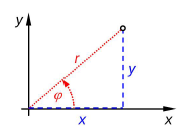
\includegraphics[width=3cm]{Images/polar}
	\end{minipage}&
	\begin{minipage}{4.2cm}
		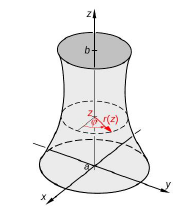
\includegraphics[width=2.6cm]{Images/zylinder}
	\end{minipage}&
	\begin{minipage}{4.2cm}
		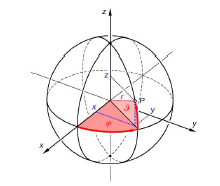
\includegraphics[width=3.2cm]{Images/kugel}
	\end{minipage}\\
	\hline
	\begin{minipage}{3cm}
		\vspace{0.1cm}
		$x=r\cos\varphi$\\
		$y=r\sin\varphi$    
		\vspace{0.1cm}
	\end{minipage}&	
	\begin{minipage}{4.2cm}
		\vspace{0.1cm}
		$x=r\cos\varphi \qquad r \geq 0$\\
		$y=r\sin\varphi \qquad 0 \leq \varphi \leq 2\pi$\\
		$z=z$
		\vspace{0.1cm}
	\end{minipage}&	
	\begin{minipage}{7.5cm}
		\vspace{0.1cm}
		$x=r\cos\varphi\cos\vartheta \quad\quad r \geq 0,$\\
		$y=r\sin\varphi\cos\vartheta \quad\quad  0\leq\varphi\leq 2\pi,$\\
		$z=r\sin\vartheta \quad\quad\quad
		-\frac{\pi}{2}\leq\vartheta\leq\frac{\pi}{2}$
		\vspace{0.1cm}
	\end{minipage}\\
	\hline
	\begin{minipage}{3cm}
		\vspace{0.1cm}
		$\begin{pmatrix}
			\cos\varphi & -r\sin\varphi\\
			\sin\varphi & r\cos\varphi
		\end{pmatrix}$
		\vspace{0.1cm}
	\end{minipage}&	
	\begin{minipage}{4.2cm}
		\vspace{0.1cm}
		$\begin{pmatrix}
			\cos\varphi & -r\sin\varphi & 0\\
			\sin\varphi & r\cos\varphi & 0\\
			0 & 0 & 1
		\end{pmatrix}$
		\vspace{0.1cm}
	\end{minipage}&	
	\begin{minipage}{7.5cm}
		\vspace{0.1cm}
		$\begin{pmatrix}
			\cos\varphi\cos\vartheta & -r\sin\varphi\cos\vartheta &
			-r\cos\varphi\sin\vartheta\\
			\sin\varphi\cos\vartheta & r\cos\varphi\cos\vartheta &
			-r\sin\varphi\sin\vartheta\\
			\sin\vartheta & 0 & r\cos\vartheta
		\end{pmatrix}$
		\vspace{0.1cm}
	\end{minipage}\\
	\hline
	$D_f = r$ &
	$D_f = r$ &
	$D_f = r^2\cos\vartheta \qquad \geq 0$\\
	\hline	
\end{tabular}
\egroup
}
\end{center}

\subsection{Schwerpunkt}
Gleichung 1 und 2 können dual getauscht werden. Dabei ist $M$ die Masse der Platte und $y_{max}$ die höhere bzw. $y_{min}$ die untere Gleichung der eingeschlossenen Fläche.
\begin{align*}
		x_S &= \frac{1}{M}\int\limits_{F}^{}x\cdot \rho(x;y)dF \xRightarrow[\text{ konst.}]{\rho} \frac{1}{F}\int\limits_{x_{min}}^{x_{max}}x[y_{max}(x) - y_{min}(x)]dx\\
		y_S &= \frac{1}{M}\int\limits_{F}^{}y\cdot \rho(x;y)dF \xRightarrow[\text{ konst.}]{\rho} \frac{1}{2F}\int\limits_{x_{min}}^{x_{max}}[y^2_{max}(x) - y^2_{min}(x)]dx
\end{align*}
\textbf{Beispiel:}
\begin{center}
	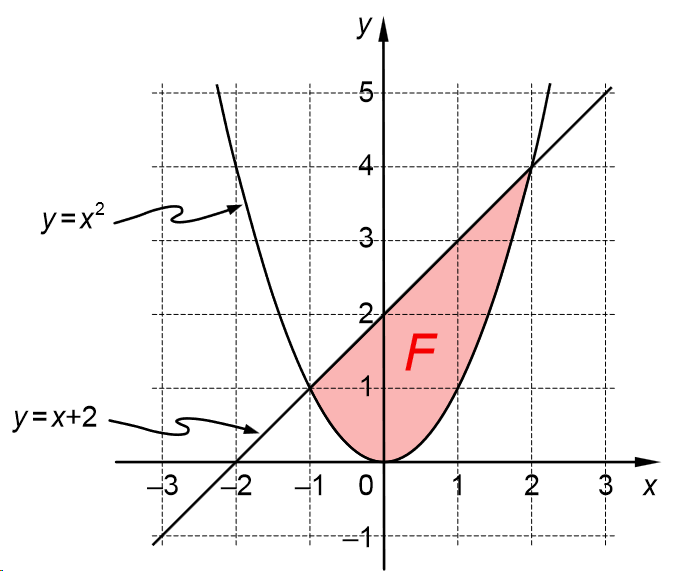
\includegraphics[width=0.5\columnwidth]{Images/schnittpunkt}\\
	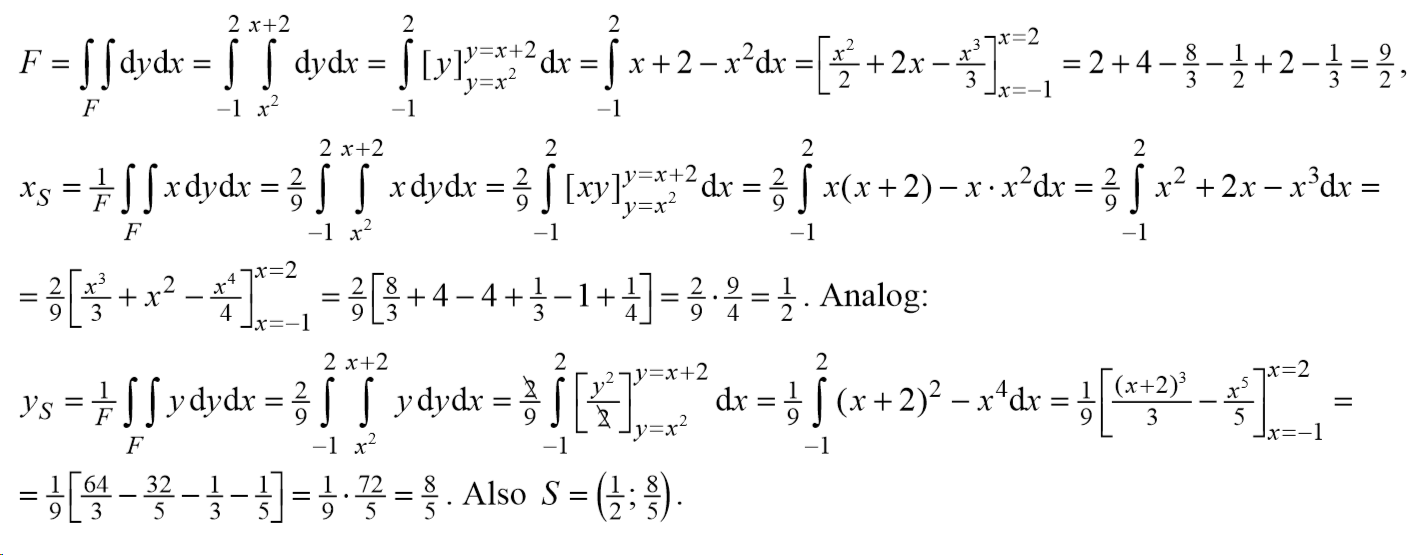
\includegraphics[width=\columnwidth]{Images/schnittpunkt1}
\end{center}



